\section{Introduzione Ai Segnali}
    \begin{itemize}
        \item {
            Deterministici: Segnale rappresentabile con funzioni analitiche e noto $\forall t$, 
            per ogni istante temporale si conosce il valore del segnale, spesso rappresentati con funzioni analitiche.
        }
        \item {
            Aleatori: Segnale rappresentabile tramite statistiche, ad esempio un rumore.
        }
    \end{itemize}
    \subsection{Classificazione di segnale in base alla continuità dei domini}
        \begin{itemize}
            \item {Dominio del tempo:
                    \begin{itemize}
                        \item{Segnale tempo continuo: $t \in \mathbb{R}$ assume con continuità tutti i valori contenuti all'interno di un intervallo}
                        \item {Segnale a tempo discreto: $t = \{ nT \} n \in \mathbb{Z} \ T=$periodo di campionamento, la variabile temporale assume solo valori discreti}
                    \end{itemize}
                    \begin{figure}[h]
                        \centering
                        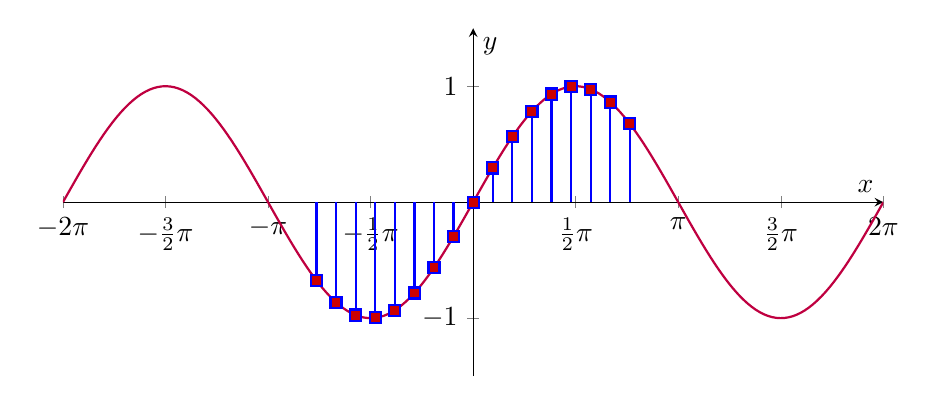
\begin{tikzpicture}
                            \begin{axis}[
                                domain=-2*pi:2*pi,
                                samples=200,
                                axis lines=middle,
                                xlabel=$x$,
                                ylabel=$y$,
                                ymin=-1.5,
                                ymax=1.5,
                                xtick={-2*pi, -3/2*pi, -pi, -1/2*pi, 0, 1/2*pi, pi, 3/2*pi, 2*pi},
                                xticklabels={$-2\pi$, $-\frac{3}{2}\pi$, $-\pi$, $-\frac{1}{2}\pi$, $0$, $\frac{1}{2}\pi$, $\pi$, $\frac{3}{2}\pi$, $2\pi$},
                                ytick={-1, 1},
                                yticklabels={$-1$, $1$},
                                width=12cm,
                                height=6cm
                            ]
                            \addplot [purple, thick] {sin(deg(x))};
                            \addplot+ [blue, thick, ycomb, samples at={-2.4,-2.1,-1.8,-1.5,-1.2,-0.9,-0.6,-0.3,0,0.3,0.6,0.9,1.2,1.5,1.8,2.1,2.4}] {sin(deg(x))};
                            \end{axis}
                        \end{tikzpicture}
                        \caption{\color{purple}{tempo continuo}, \color{blue}{tempo discreto:$T=0.3$}}
                        \label{fig:Dominio del tempo}
                    \end{figure}                        
            }
            \item {Dominio dell'ampiezza (spazio):
                    \begin{itemize}
                        \item{Segnale ad ampiezza continua: $x_{(t)}\ continua$, la grandezza fisica del segnale assume con continuità tutti i valori all'interno di un intervallo}
                        \item {Segnale ad ampiezza discreta: $x_{(t)}\ discreta$,se restringo l'intervallo posso renderla continua, la grandezza fisica può assumere solo valori discreti}
                    \end{itemize}
                    \begin{figure}[H]
                        \centering
                        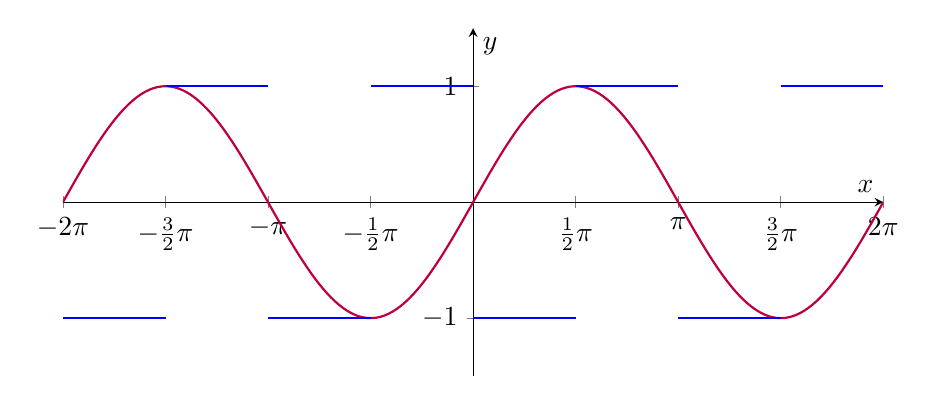
\begin{tikzpicture}
                            \begin{axis}[
                                domain=-2*pi:2*pi,
                                samples=200,
                                axis lines=middle,
                                xlabel=$x$,
                                ylabel=$y$,
                                ymin=-1.5,
                                ymax=1.5,
                                xtick={-2*pi, -3/2*pi, -pi, -1/2*pi, 0, 1/2*pi, pi, 3/2*pi, 2*pi},
                                xticklabels={$-2\pi$, $-\frac{3}{2}\pi$, $-\pi$, $-\frac{1}{2}\pi$, $0$, $\frac{1}{2}\pi$, $\pi$, $\frac{3}{2}\pi$, $2\pi$},
                                ytick={-1, 1},
                                yticklabels={$-1$, $1$},
                                width=12cm,
                                height=6cm
                            ]
                            \addplot [purple, thick] {sin(deg(x))};
                            \addplot [blue, thick, jump mark left] coordinates {
                                (-2*pi,-1) (-3/2*pi,1) (-pi,-1) (-1/2*pi,1) (0,-1) (1/2*pi,1) (pi,-1) (3/2*pi,1) (2*pi,-1)
                            };
                            \end{axis}
                        \end{tikzpicture}
                        \caption{\color{purple}{ampiezza continua}, \color{blue}{ampiezza discreta}}
                        \label{fig:dominio dell'ampiezza}
                    \end{figure}
                    }
        \end{itemize}
        Possiamo costruire una tabella per categorizzare le tipologie di segnali:
        \begin{table}[h]
            \centering
            \begin{tabular}{c|cccc}
            Segnale   & \multicolumn{1}{c|}{Continuo}     & Discreto          & $t$ &  \\ \cline{1-4}
            Continua  & \multicolumn{1}{c|}{Analogico}   & Sequenza/Digitale &       &  \\ \cline{1-3}
            Discreta  & \multicolumn{1}{c|}{Quantizzato} & Binario           &       &  \\
            $x_{(t)}$ &                                  &                   &       & 
            \end{tabular}
        \end{table}
